%\title{LaTeX Portrait Poster Template}
%%%%%%%%%%%%%%%%%%%%%%%%%%%%%%%%%%%%%%%%%
% a0poster Portrait Poster
% LaTeX Template
% Version 1.0 (22/06/13)
%
% The a0poster class was created by:
% Gerlinde Kettl and Matthias Weiser (tex@kettl.de)
% 
% This template has been downloaded from:
% http://www.LaTeXTemplates.com
%
% License:
% CC BY-NC-SA 3.0 (http://creativecommons.org/licenses/by-nc-sa/3.0/)
%
%%%%%%%%%%%%%%%%%%%%%%%%%%%%%%%%%%%%%%%%%

%----------------------------------------------------------------------------------------
% PACKAGES AND OTHER DOCUMENT CONFIGURATIONS
%----------------------------------------------------------------------------------------

\documentclass[final]{beamer}
\usepackage[scale=1.40]{beamerposter}  

\usepackage{algorithm}
\usepackage{algorithmicx}
\usepackage{algpseudocode}
\usepackage{multicol} % This is so we can have multiple columns of text side-by-side
\columnsep=100pt % This is the amount of white space between the columns in the poster
\columnseprule=0pt % This is the thickness of the black line between the columns in the poster
\usepackage{tikz}
\usetikzlibrary{calc}

% put color to \boxed math command
\newcommand*{\boxcolor}{orange}
\makeatletter
\renewcommand{\boxed}[1]{\textcolor{\boxcolor}{%
\tikz[baseline={([yshift=-1ex]current bounding box.center)}] \node [rectangle, minimum width=1ex,rounded corners,draw] {\normalcolor\m@th$\displaystyle#1$};}}
 \makeatother



%\usepackage{empheq}
\usepackage[most]{tcolorbox}

\tcbset{colback=yellow!10!white, colframe=red!50!black, 
        highlight math style= {enhanced, %<-- needed for the ’remember’ options
            colframe=red,colback=red!10!white,boxsep=0pt}
        }

\definecolor{blue}{RGB}{0,0,255}
\usepackage{tcolorbox}

% \usepackage[bitstream-charter]{mathdesign}
\usepackage[authoryear,round]{natbib}
\usepackage{bbm}
\usepackage{xargs} 
\usepackage{amssymb,amsthm,bm}
%\usepackage{mathtools}
%\usepackage{xargs}
%\usepackage{stmaryrd} 

\bibliographystyle{plainnat}
\usepackage{graphicx} % Required for including images
\graphicspath{{figures/}} % Location of the graphics files
\usepackage{booktabs} % Top and bottom rules for table
%\usepackage[font=small,labelfont=bf]{caption} % Required for specifying captions to tables and figures
%\usepackage{amsfonts, amsmath, amsthm, amssymb,bm} % For math fonts, symbols and environments
\usepackage{wrapfig} % Allows wrapping text around tables and figures

\usepackage{cmbright}
%\usepackage{avant}
%\usepackage{tikz}
%\usepackage[T1]{fontenc}
%\usepackage[utf8]{inputenc}
%\usepackage[font=small,labelfont=bf,tableposition=top]{caption}

\renewcommand{\familydefault}{\sfdefault}

\usepackage{mdframed}
%\theoremstyle{definition}
%\newtheorem{defn}{Definition} % definition numbers are dependent on theorem numbers
%\newtheorem*{exmp}{Example} % same for example numbers
%\usepackage{lipsum}%
%  {
%      \theoremstyle{plain}
%      \newtheorem{assumption}{M}
%      \newtheorem{lemma}{Lemma}
%      \newtheorem{remark}{Remark}
%      \newtheorem{prop}{Proposition}
%      \newtheorem{assumption_saem}{ISAEM}
%      \newtheorem{assumption_rm}{SA}
%      \newtheorem{assumption_iem}{iEM}
%      \newtheorem{assumption_imcem}{IMCEM}
%      \newtheorem{assumption_expo}{E}
%  }
\newmdtheoremenv{theo}{Theorem}
\newmdtheoremenv{coro}{Corollary}
\newmdtheoremenv{lem}{Lemma}


\usepackage{shortcuts_OPT}
  \definecolor{myorange}{rgb}{1,0.699,0.0625}

\begin{document}

{~\hspace{6cm}\begin{tikzpicture}[remember picture, overlay]
     \node [anchor=north east, inner sep=3cm, yshift=-3cm]  at (current page.north east)
     {
\includegraphics[height=6cm]{images/logo_baidu.jpeg}
       
\includegraphics[height=5cm]{images/logo_cuhk.png}~~
     
\includegraphics[height=5cm]{images/logo_x.jpg}};
  \end{tikzpicture}}
  
  \begin{tikzpicture}[remember picture, overlay]
     \node [inner sep=3cm, yshift=2cm]  at (current page.south)
     {\large The 33rd International Conference on Algorithmic Learning Theory, Paris, France};
%          \node [inner sep=3cm,xshift=16cm, yshift=2cm]  at (current page.south west)
%     {belhal.karimi@polytechnique.edu, htwai@cuhk.edu.hk};    
  \end{tikzpicture}
%----------------------------------------------------------------------------------------
% POSTER HEADER 
%----------------------------------------------------------------------------------------

% The header is divided into two boxes:
% The first is 75% wide and houses the title, subtitle, names, university/organization and contact information
% The second is 25% wide and houses a logo for your university/organization or a photo of you
% The widths of these boxes can be easily edited to accommodate your content as you see fit

\begin{minipage}[b]{0.9\linewidth}
\Huge  \textbf{Minimization by Incremental Stochastic Surrogate Optimization for Large Scale Nonconvex Problems
}\\[1cm]  
\LARGE \textbf{Belhal Karimi$^{1}$, Hoi-To Wai$^{2}$, Eric Moulines$^{3}$ and Ping Li$^{1}$}\\[0.5cm] % Author(s)
\LARGE Baidu Research$^1$, Chinese University~of Hong Kong$^2$, Ecole Polytechnique$^3$ \\[0.4cm] % University/organization
\large \texttt{}
\end{minipage}
%


\vspace{1cm} % A bit of extra whitespace between the header and poster content

%----------------------------------------------------------------------------------------


%----------------------------------------------------------------------------------------
% ABSTRACT
%----------------------------------------------------------------------------------------




%----------------------------------------------------------------------------------------
% INTRODUCTION
%----------------------------------------------------------------------------------------

%\color{SaddleBrown} % SaddleBrown color for the introduction
%\color{Navy} % Navy color
%\color{opticlimb}
%\color{Navy} % Navy color for the abstract

    \begin{columns}[t]

      \begin{column}{.25\linewidth}

  \vspace{-2.5cm}
\begin{tcolorbox}[colback=white!5!white,colframe=white,coltitle=blue!75!black,fonttitle=\sffamily\bfseries\large,title= \center Large Scale Optimization]
{\color{blue!75!black} \noindent\rule[0.5ex]{\linewidth}{4pt}}

$\bullet$  \textbf{Objective:} \emph{Constrained} minimization problem of a finite sum of  functions:
\beq \label{eq:opt}
\min_{ \param \in \Param }~ {\cal L} ( \param ) \eqdef \frac{1}{n} \sum_{i=1}^n {\cal L}_i( \param) \eqsp,
\eeq
where ${\cal L} _i: \rset^p \to \rset$ is bounded from below and is (possibly) nonconvex and include a nonsmooth penalty.
$\bullet$ The gap $\widehat{e}(\param ; \{ \op_i \}_{i=1}^n )$ is L-smooth.
\begin{mdframed}[backgroundcolor=myorange!8!white,roundcorner=0.5em,linecolor=white]
\textbf{Asymptotic Stationary Point Condition}: 
\[
f'( \param, {\bm d} ) \eqdef \lim_{ t \rightarrow 0^+ } \frac{ f ( \param + t {\bm d} ) - f( \param ) }{ t }  \geq 0.
\]
\end{mdframed}\vspace{.4cm}



 
\vspace{.1cm}
\end{tcolorbox}


\begin{tcolorbox}[colback=white!5!white,colframe=white,coltitle=blue!75!black,fonttitle=\sffamily\bfseries\large,title=\center The MISO Method~\citep{mairal2015miso}]
{\color{blue!75!black} \noindent\rule[0.5ex]{\linewidth}{4pt}}

$\bullet$ MISO has been proposed in ~\citep{mairal2015miso}
\begin{mdframed}[backgroundcolor=gray!3,roundcorner=0.5em]
 
$\bullet$  Initialize the majorizing surrogate functions
$$
\tafctdet{i}{0}{ \param } \eqdef \sur{i}{\param}{\hp{0}},~i \in [n].
$$
$\bullet$ For $k > 0$:

\hspace*{10mm} $\bullet$ Pick $i_k$ uniformly from $[n]$.

\hspace*{10mm} $\bullet$ Update $\tafctdet{i}{k+1}{\param}$ as: 
\beq \notag
\tafctdet{i}{k+1}{\param} = \begin{cases}
\sur{i}{\param}{\hp{k}}, & \text{if}~i = i_k \\
\tafctdet{i}{k}{\param}, & \text{otherwise}.
\end{cases}
\eeq

\hspace*{10mm} $\bullet$ Set $\hp{k+1} \in \argmin \limits_{ \param \in \Param }  \frac{1}{n} \sum_{i=1}^n \tafctdet{i}{k+1}{\param}$.

$\bullet$  \textbf{Return}: $\hp{k+1}$.

\end{mdframed}

\end{tcolorbox}



\begin{tcolorbox}[colback=white!5!white,colframe=white,coltitle=blue!75!black,fonttitle=\sffamily\bfseries\large,title= \center An Intractability for Latent Data Models]
{\color{blue!75!black} \noindent\rule[0.5ex]{\linewidth}{4pt}}

$\bullet$ Case when the surrogate functions computed in MISO \textbf{are not tractable}.
$\bullet$ Surrogate is expressed as an integral over a set of latent variables $z$.
\vspace{.1cm}
\begin{tcolorbox}[colback=red!5!white,colframe=red!75!black]
\begin{equation}\label{eq:integralsurrogate}
\sur{i}{\param}{\op} \eqdef \int_{\Zset}{\rsur{i}{\param}{\op}{z_i}  p_i(z_i ; \op)\mu_i(dz_i)} \eqsp.
\end{equation}
\end{tcolorbox}  

$\bullet$ Our scheme is based on the computation of $\ssur{i}{\param}{\op}{ \{ z_m \}_{m=1}^{M}}$, a Monte Carlo approximation of the surrogate function $\sur{i}{\param}{\op}$ defined by \eqref{eq:integralsurrogate} such that:
\begin{tcolorbox}[colback=green!5!white,colframe=green!75!black]
\beq \label{eq:ssur}  
\ssur{i}{\param}{\op}{ \{ z_m \}_{m=1}^{M}} \eqdef \frac{1}{M} \sum_{m=1}^{M} \rsur{i}{\param}{\op}{z_m}\eqsp,
\eeq
\end{tcolorbox}
where $\{z_i^{m}\}_{m=0}^{M-1}$ is a Monte Carlo batch.

\vspace{.1cm}
\end{tcolorbox}
      \end{column}
      \begin{column}{.51\linewidth}

\vspace{-2.5cm}


\begin{tcolorbox}[colback=white!5!white,colframe=white,coltitle=blue!75!black,fonttitle=\sffamily\bfseries\large,title=\center MISSO: Minimization by Incremental Stochastic Surrogate Optimization]
{\color{blue!75!black} \noindent\rule[0.5ex]{\linewidth}{4pt}}
\textbf{Idea}: We replace the expectation in \eqref{eq:integralsurrogate} by a \emph{Monte Carlo} integration and then optimizes the objective function in an incremental manner..
 
 \begin{figure}[H]
\centering
        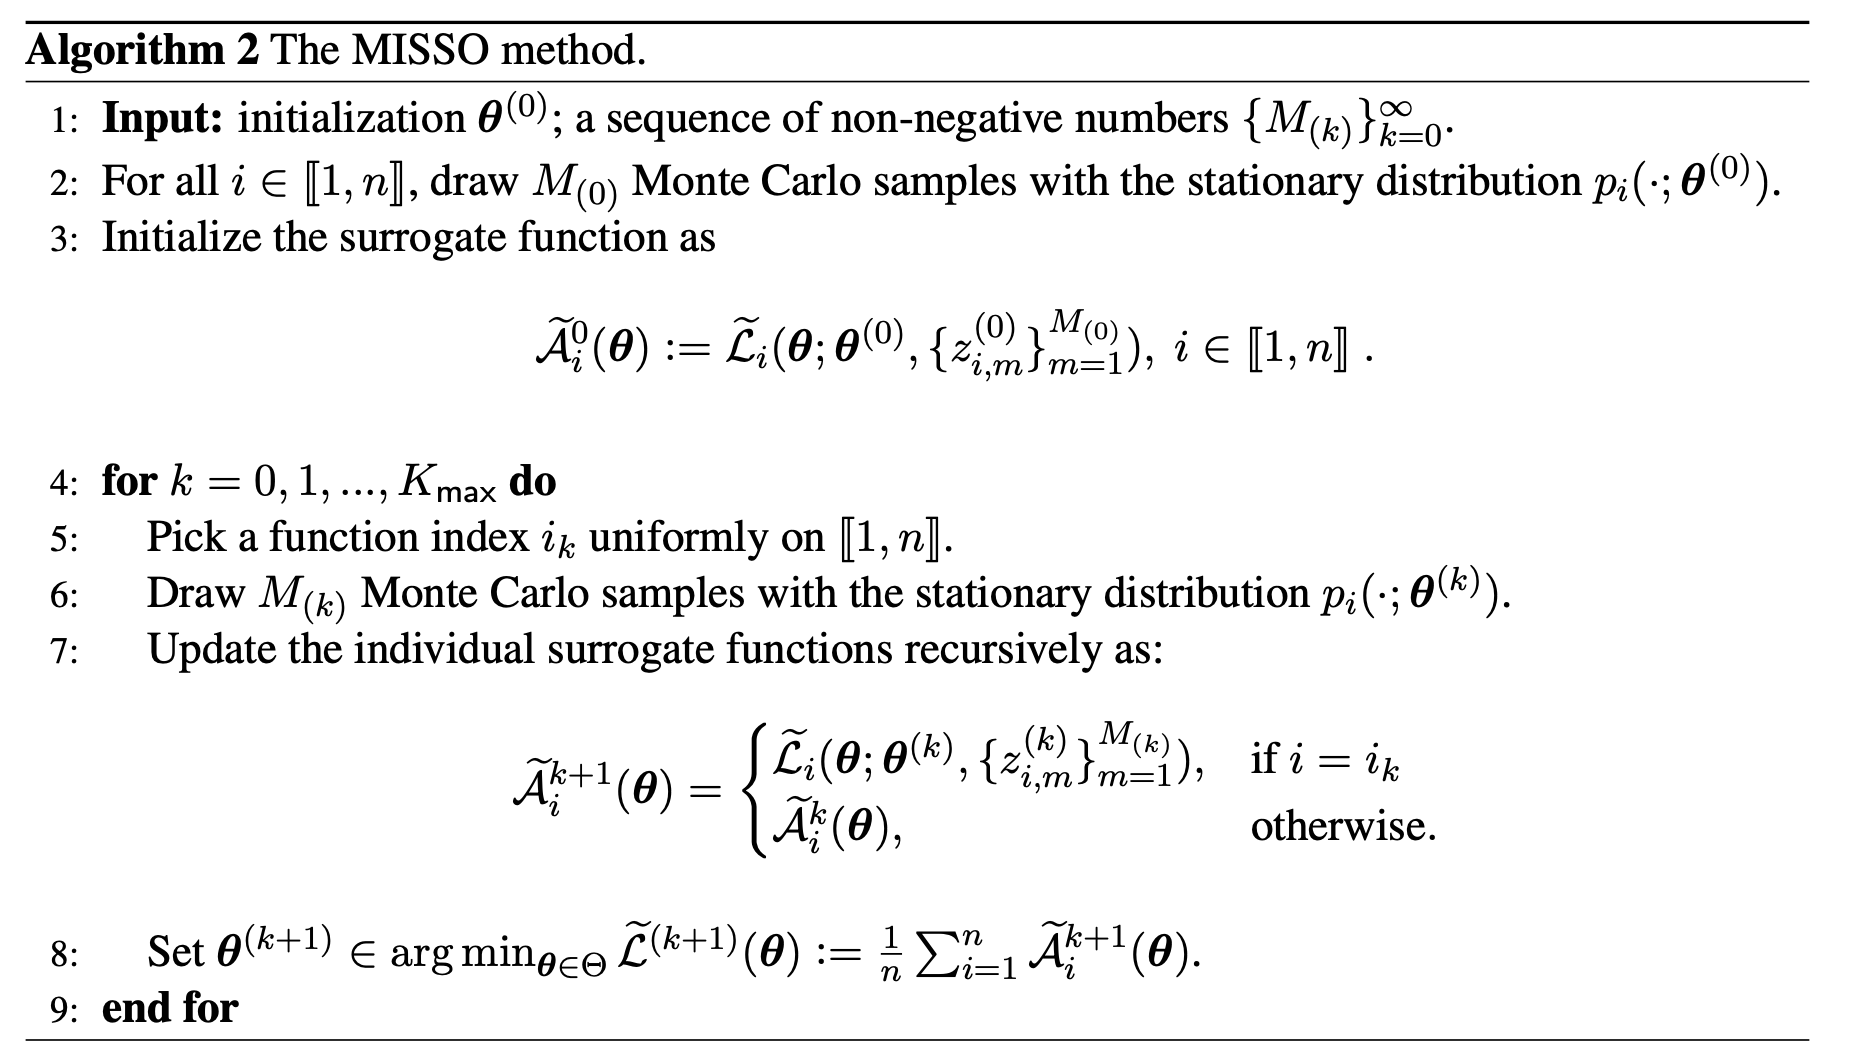
\includegraphics[width=1.\textwidth]{fig/missoalgo}
\end{figure}

\end{tcolorbox}\vspace{-.3cm}


\begin{mdframed}[backgroundcolor=white,roundcorner=0.5em,linecolor=white]
\begin{center}
{\color{red!75!black} 
%\textbf{
%\Large Large datasets $\Rightarrow$ incremental (iEM) or variance reduced (sEM-VR and fiEM) variants.}

\large \textbf{How does this Monte Carlo Approximation affects the convergence rate?}\vspace{.8cm}
}
\end{center}
\end{mdframed}



\vspace{-.2cm}
\begin{tcolorbox}[colback=white!5!white,colframe=white,coltitle=green!50!black,fonttitle=\sffamily\bfseries\large,title=\center Global Convergence Analysis]
{\color{green!50!black} \noindent\rule[0.5ex]{\linewidth}{4pt}}
 
$\bullet$ We bound the \textbf{{\color{green!50!black} Monte Carlo noise }} by some constants using the notion of metric entropy (or bracketing number) see~\citet{van2000asymptotic}: $\EE \left[\underset{f \in \mathcal{F}}{ \sup } \left|\frac{1}{M} \sum_{i=1}^{M} f\left(z_{i,m}\right)-\EE[f(z_i)]\right| \right] \leq \frac{C L}{\sqrt{M}} $.

$\bullet$ \textbf{Convergence Analysis}: Assume \textbf{{\color{red!75!black} $\sur{i}{\param}{\op} \geq {\cal L}_i( \param )$ }} and the error gap follows  \textbf{{\color{green!75!black} $\| \grd \widehat{e}(\param; \{ \op_i \}_{i=1}^n)  \|^2 \leq 2 L\!~ \widehat{e}(\param; \{ \op_i \}_{i=1}^n)$ }}
\vspace{.3cm}
\begin{mdframed}[backgroundcolor=myorange!8!white,roundcorner=0.5em,linecolor=white]
\textbf{Theorem (MISSO Finite-Time Convergence)}
For any $K_{\max} \geq 1$, $K \sim {\cal U}([0,K_{\max}-1])$ independent of the $\{i_k\}_{k=0}^{K_{\max}}$, we have the \textbf{global rate}:\vspace{-.2cm}
{
\beq
 \EE \big[ \| \grd \eSur{K}{\hp{K}} \|^2 \big]  \leq \frac{\Delta_{( K_{\sf max} )}}{K_{\sf max}} \ \  \textrm{and} \ \  \EE[ g_-( \hp{K} ) ]  \leq \sqrt{\frac{ \Delta_{( K_{\sf max} )} }{ K_{\sf max} }} + \frac{C_{\sf gr}}{K_{\sf max}}  \overline{M}_{(K_{\sf max})} \eqsp.
\eeq\vspace{-.7cm}
}
where
$$\Delta_{( K_{\sf max} )} \eqdef 2 n L \EE[  \sumSur{0}{\hp{0}} - \sumSur{K_{\sf max}}{\hp{K_{\sf max}}} ] +  4 L C_{\sf r} \overline{M}_{(K_{\sf max})} \eqsp.$$
\end{mdframed}

\end{tcolorbox}

\vspace{.5cm}


%\begin{tcolorbox}[colback=white!5!white,colframe=white,coltitle=red!75!black,fonttitle=\sffamily\bfseries\large,title=\center sEM-VR/fiEM are Scaled Gradient Methods and Faster than iEM]
%{\color{red!75!black} \noindent\rule[0.5ex]{\linewidth}{4pt}}
%$\bullet$ Unlike iEM, the sEM-VR and fiEM methods can be analyzed as \textbf{\textit{scaled gradients}} methods. Consider:\vspace{-.2cm}
%%\textbf{{\color{green!75!black} smooth}} Lyapunov function as:
%$$ 
%\min_{ {\bss} \in \Sset }~  V ( {\bss} ) \eqdef \overline\calL( \op(\bss) ) = 
%\Pen (  \op(\bss) ) + \frac{1}{n} \sum_{i=1}^n {\cal L}_i (  \op(\bss) )\vspace{-.2cm}
%$$
%$\bullet$ \textbf{\color{blue!75!black}Variance-reduced scaled gradient}: the sE-step update $\hat{\bss}^{(k)}$ by {\color{red!75!black}$\hat{\bss}^{(k)} -  \StocEstep^{(k+1)}$}, observe\vspace{.3cm}
%$$ 
%\pscal{ \EE[ {\color{red!75!black}\hat{\bss}^{(k)} -  \StocEstep^{(k+1)}} ] }{ \grd V(\hat\bss^{(k)} ) } \geq \upsilon_1 \!~ \| \EE[ \hat{\bss}^{(k)} -  \StocEstep^{(k+1)} ] \|^2 \geq \upsilon_2 \!~ \| \grd V(\hat{\bss}^{(k)}) \|^2~~~\text{for some}~\upsilon_1, \upsilon_2 > 0.\vspace{.3cm}
%$$
%
%$\therefore$ the sEM-VR/fiEM methods are \textbf{variance-reduced, scaled gradient} updates of the sufficient statistics.\vspace{.3cm}
%
%$\bullet$ \textbf{Convergence Analysis}: with exponential family model, \textbf{\color{red!75!black}the function 
%$V ( {\bss} )$ is $\overline{L}_{\sf v}$-smooth}, \vspace{-.7cm}
%   \begin{columns}[t]
%      \begin{column}{.5\linewidth}
%\begin{mdframed}[backgroundcolor=myorange!8!white,roundcorner=0.5em,linecolor=white]
%\textbf{Theorem (sEM-VR)}
%$\gamma = \frac{\mu \upsilon_{\min} }{ \overline{L}_{\sf v} n^{2/3}}$ \& epoch $m = \frac{n }{2 \mu^2 \upsilon_{\min}^2 +\mu }$:
%{
%\beq \notag
%\EE[ \| \grd V( \hs{K} ) \|^2 ] \leq \boxed{ n^{\frac{2}{3}} \!~ \frac{2 \overline{L}_{\sf v} }{\mu K_{\sf max}}} \frac{ \upsilon_{\max}^2 }{ \upsilon_{\min}^2 } \!~ \EE[ V( \hs{0} ) - V( \hs{K_{\sf max}}) ] .
%\eeq\vspace{-.5cm}
%}
%\end{mdframed}
%
%      \end{column}
%
%
%      \begin{column}{.5\linewidth}
%\begin{mdframed}[backgroundcolor=myorange!8!white,roundcorner=0.5em,linecolor=white]
%\textbf{Theorem (fiEM)}
%$\gamma = \frac{\upsilon_{\min}}{\alpha \overline{L}_{\sf v} n^{2/3}}$ \& $\alpha = \max\{ 6, 1 + 4 \upsilon_{\min} \}$:
%{
%\beq \notag
%\EE[ \| \grd V( \hs{K} ) \|^2 ] \leq \boxed{n^{\frac{2}{3}} \!~ \frac{ \alpha^2 \overline{L}_{\sf v} }{K_{\sf max}}  \frac{ \upsilon_{\max}^2 }{ \upsilon_{\min}^2 } }\EE \big[ V( \hs{0} ) - V( \hs{K_{\sf max}} ) \big] .
%\eeq\vspace{-.5cm}
%}
%\end{mdframed}
%
%      
%      \end{column}
%            \end{columns}      
%\end{tcolorbox}
%


      \end{column}
            \begin{column}{.225\linewidth}


\vspace{-2.5cm}
\begin{tcolorbox}[colback=white!5!white,colframe=white,coltitle=yellow!50!black,fonttitle=\sffamily\bfseries\large,title=\center Logistic Regression on Hemorrhage dataset]
{\color{yellow!50!black} \noindent\rule[0.5ex]{\linewidth}{4pt}}

$\bullet$  \textbf{Goal}: Logistic Regression \textbf{with missing values} on Traumabase (severe hemorrhage):
\beq\notag
p_i(y_i|z_i) =  S({\bm \delta}^\top \bar{z}_i)^{y_i} \left(1 - S({\bm \delta}^\top \bar{z}_i)\right)^{1-y_i}\eqsp,
\eeq
$\bullet$ $16$ quantitative measurements, like BMI, age, blood pressure, heart rate at different stages after the accident on $6384$ patients
$\bullet$ \textbf{MISSO is an incremental MCEM in this case}

\begin{figure}[H]
\centering
    \mbox{
        \includegraphics[width=0.5\textwidth]{fig/logisticdelta.eps}
        \includegraphics[width=0.5\textwidth]{fig/logisticbeta.eps}
    }
\end{figure} 


 
\end{tcolorbox}


\begin{tcolorbox}[colback=white!5!white,colframe=white,coltitle=yellow!50!black,fonttitle=\sffamily\bfseries\large,title=\center Bayesian Neural Networks using MISSO]
{\color{yellow!50!black} \noindent\rule[0.5ex]{\linewidth}{4pt}}

$\bullet$  \textbf{Goal}: Train Bayesian variants of LeNet-5 and ResNet-18 on MNIST and CIFAR10:

$\bullet$ Variational inference and the ELBO loss to fit Bayesian Neural Networks on different datasets.
$\bullet$ \textbf{MISSO is an incremental VI in this case}

\begin{figure}[H]
\centering
    \mbox{
        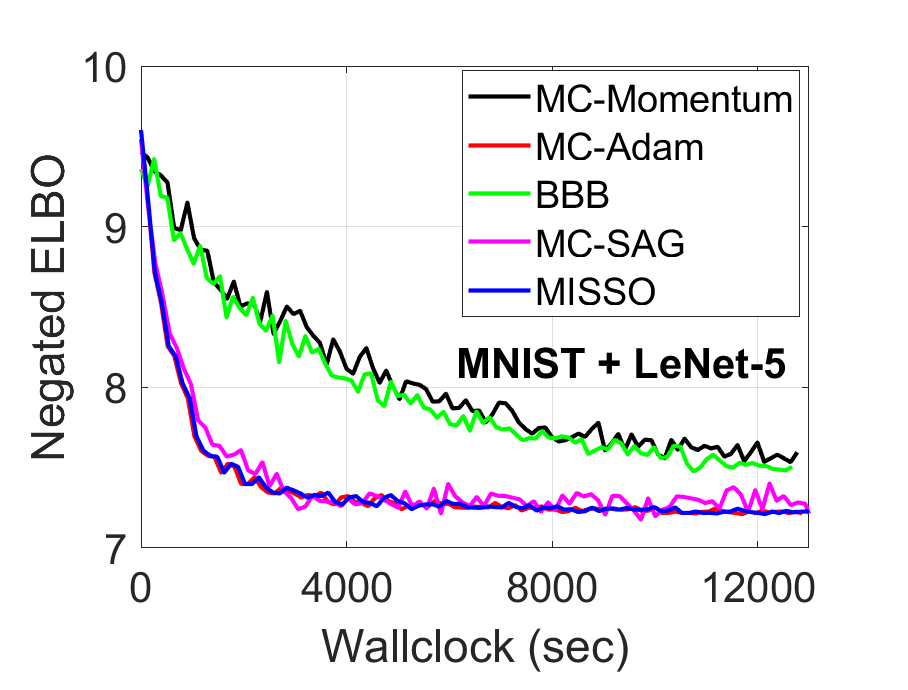
\includegraphics[width=0.5\textwidth]{fig/mnist.eps}
        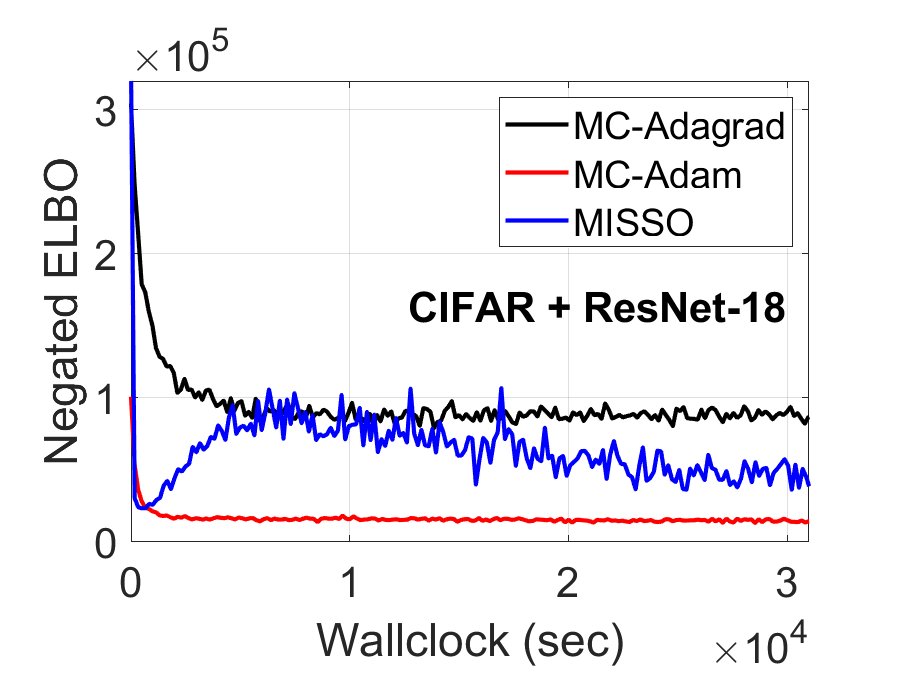
\includegraphics[width=0.5\textwidth]{fig/cifar.eps}
    }
\label{fig:gmmplots}
\end{figure} 

\end{tcolorbox}

\begin{tcolorbox}[colback=white!5!white,colframe=white,coltitle=blue!75!black,fonttitle=\sffamily\bfseries\large,title=\center References]
{\color{blue!75!black} \noindent\rule[0.5ex]{\linewidth}{4pt}}
\vspace{-1.5cm}
\small
\nocite{*} % Print all references regardless of whether they were cited in the poster or not
\bibliography{references.bib}
\end{tcolorbox}

      \end{column}
      \end{columns}


%----------------------------------------------------------------------------------------
% ACKNOWLEDGEMENTS
%----------------------------------------------------------------------------------------

%\section*{Acknowledgements}

%\includegraphics[width=15cm]{opticlimb.png}\\


%----------------------------------------------------------------------------------------

\end{document}